\documentclass{article}
\usepackage[preprint]{tmlr}
\usepackage[T1]{fontenc}
\usepackage[utf8]{inputenc}
\usepackage{graphicx}
\usepackage{booktabs}
\usepackage{amsmath,amssymb}
\usepackage{hyperref}
\usepackage{url}
\usepackage{xcolor}
\graphicspath{{figures/}}
\definecolor{linkblue}{HTML}{1D4E89}
\hypersetup{colorlinks=true, linkcolor=linkblue, citecolor=linkblue, urlcolor=linkblue,
            pdftitle={Hiding the Name Does Not Hide the Judge: Self-Preference of LLM Judges on Real Shopping Answers},
            pdfauthor={Vahit FERYAD}}

\title{Hiding the Name Does Not Hide the Judge:\\ Self-Preference of LLM Judges on Real Shopping Answers}

\author{\name Vahit FERYAD \email \href{mailto:vahit.feryat@gmail.com}{vahit.feryat@gmail.com}\\
\addr Independent researcher, Istanbul, T\"urkiye\\
\addr ORCID: \href{https://orcid.org/0000-0002-3282-339X}{0000-0002-3282-339X}\\
\addr Code and data: \href{https://github.com/vahit19/verdict-gate/tree/main/studies/judge_self_preference}{github.com/vahit19/verdict-gate}}

\begin{document}
\maketitle

\begin{abstract}
Large language model (LLM) judges are often drawn from the same model families whose answers they grade, and hiding which system wrote each answer is the usual safeguard. We test this safeguard on a public dataset of 8,794 answers from four AI shopping assistants, released by a study whose own judge was one of the graded engines. A character n-gram classifier names the engine behind an anonymized answer 98.0\% of the time on questions it never saw, against 25\% by chance. We then let the three models that wrote the answers judge them in 2,160 order-balanced pairwise comparisons on 120 questions. Relative to a judge from the third family, the Gemini judge favors Gemini's answers by 50 points (95\% interval 45 to 56) and the ChatGPT judge favors ChatGPT's by 26 (20 to 32). The Claude judge does not favor Claude ($-6$, from $-12$ to 0). Told that one of two answers is its own, Gemini picks its own 92\% of the time and ChatGPT 85\%. Rewriting all answers into one plain style with a fourth model family keeps 99\% of their checkable claims, leaves the preference unchanged and leaves recognition high (83\% and 86\%). Showing the judge only the extracted claims reduces the preference to $+24$ and $+7$. Across judges and input views, recognition and preference move together. A judge pipeline should therefore not let a model family judge a comparison that contains its own answer, and should give judges claims rather than prose.
\end{abstract}

\section{Introduction}
\label{sec:intro}

LLM judges decide what many evaluation pipelines report and what many products publish: which answer is better, whether a claim is supported, which system ranks first. Self-preference, the tendency of a judge to rate its own outputs above what other judges would give them, is a documented weakness of such judges \citep{zheng2023judging,panickssery2024llm,wataoka2024self}. In practice the judge often belongs to one of the model families under comparison, because the strongest available judges are the same frontier models whose outputs are being tested. The usual safeguard is to hide which system wrote which answer.

A recent study of AI shopping assistants shows this setting clearly \citep{productai2026divergence}. It asked four engines, ChatGPT, Claude, Gemini and Perplexity, each on a free and a paid tier, the same 220 pre-registered shopping questions five times, and used an LLM judge to classify factual conflicts among the answers. The judge was Claude, one of the engines under measurement. The authors called this ``a real conflict of interest, not a solved problem'', hid and re-shuffled engine identities for every judgment, noted that writing style could still reveal identity, and released every answer under a CC BY 4.0 license. Whether the safeguard works on answers like these is not known. Prior measurements of self-preference used generations produced for the experiment, and we cannot tell from them whether hiding names protects a same-family judge on real production answers, or which change to the judge's input would remove the preference if it does not.

This paper measures both on the released answers. We show that the engine behind an anonymized answer can be identified almost always, and that two of the three judges favor their own family by large margins while the third does not. The two self-favoring judges also recognize their own answers. Rewriting answers into a common style does not reduce the preference, while reducing answers to their checkable claims does. We also show that the choice of judge decides which engine ranks first. The measurements give two checks that a judge pipeline can run in code.

\section{Related work}
\label{sec:related}

\paragraph{Biases of LLM judges.} \citet{zheng2023judging} listed self-enhancement among the biases of LLM judges, together with position and verbosity bias, in their study of MT-Bench and Chatbot Arena. Position bias is the reason we present every pair in both orders.

\paragraph{Why judges favor themselves.} \citet{panickssery2024llm} showed that LLMs can distinguish their own generations from those of other models and of humans. Varying this ability by fine-tuning, they found that the strength of self-recognition correlates linearly with the strength of self-preference. \citet{wataoka2024self} found that judges give higher scores to outputs with lower perplexity under the judge, and argued that self-preference arises because judges prefer text that is familiar to them.

\paragraph{Mitigation by judge choice.} \citet{verga2024replacing} replaced a single large judge with a panel of smaller judges from different model families; the panel outperformed the single judge while reducing intra-model bias and cost.

These studies leave three questions open for a deployed pipeline. Does hiding names prevent recognition on real answers to a third party's questions? Does recognition rest on style or on content? And can a change to the judge's input, rather than to the choice of judge, reduce the preference?

\section{Methods}
\label{sec:methods}

\paragraph{Answers.} The dataset \citep{productai2026divergence} contains 8,794 answers: 220 questions in nine product categories, four engines, a free and a paid tier for each, and five samples per configuration, captured on 2026-09-01 through each provider's API with web search enabled. The source study excluded three questions from scoring because provider outages left them incomplete, and we exclude the same three. For the classifier we use every non-empty answer (8,793; one Gemini answer is empty). For the judge experiments we use the free-tier answers of the three engines that have a matching judge model, sample 0, on 120 questions drawn at random (seed 0) from the scored questions with all three answers present.

\paragraph{Classifier.} A logistic regression ($C = 4$) on TF-IDF features of character 2- to 5-grams (word-bounded, sublinear term frequency, minimum document frequency 3, at most 200,000 features) predicts which of the four engines wrote an answer. Five-fold cross-validation is grouped by question, so every test answer comes from a question absent from training. We report accuracy on three views of each answer (raw, links and formatting removed, claims only) and on a control in which engine labels are shuffled within each question.

\paragraph{Judges.} The judges are the models that wrote the free-tier answers: \texttt{claude-sonnet-5}, \texttt{gpt-5.6-luna} and \texttt{gemini-3.6-flash}. As a second judge for each family we use the paid-tier models \texttt{claude-opus-5}, \texttt{gpt-5.6-sol} and \texttt{gemini-3.1-pro-preview}, applied to the same free-tier answers. All models were called through OpenRouter with low reasoning effort, and the model name returned with each call matched the requested model in every call. Before judging, links are replaced by their anchor text, bare URLs and citation markers are removed, and each answer is truncated to 6,000 characters. This removes literal fingerprints such as the tracking parameter \texttt{utm\_source=openai}, which appears in 77.8\% of ChatGPT's raw answers.

\paragraph{Pairwise preference.} For each question and each of the three engine pairs, each judge reads the question and two answers and picks the answer that is more factually reliable for the shopper (Appendix~\ref{app:prompts}). Every pair is shown in both orders, which gives 2,160 judgments per input view. For one question, the win score of answer $X$ under judge $J$ is the share of the two orders in which $J$ picked $X$.

\paragraph{Self-preference.} For a family $F$ and an opponent $O$, let $N$ be the third family, the one that wrote neither answer. The self-preference of $F$ against $O$ is the mean over questions of the win score of $F$'s answer under judge $F$ minus its win score under judge $N$. A family's self-preference averages the two opponents. Without ground truth no judge is a neutral reference; the third-family judge is the closest substitute that has no answer of its own in the pair.

\paragraph{Self-recognition.} Each judge sees its own answer and another engine's answer to the same question, is told that exactly one of them was written by it in a separate session, and names which. Two opponents and two orders give four judgments per question and judge, and 1,440 judgments per input view. Chance is 50\%.

\paragraph{Input views.} In the \emph{full} view the judge sees the cleaned answer. In the \emph{rewritten} view a model from a fourth family, \texttt{qwen3-235b-a22b-2507}, has rewritten the answer into plain paragraphs, with instructions to keep every product name, model number, price, number, recommendation and claim exactly, including wrong ones, and to remove all formatting. We measure how many of each answer's checkable claims survive the rewrite. In the \emph{claims} view the judge sees only the checkable tokens of the answer (prices, numbers with units and alphanumeric model numbers), de-duplicated and sorted, so that neither order nor wording survives.

\paragraph{Statistics.} Intervals are 95\% percentile bootstrap intervals over questions with 5,000 resamples. We report the Pearson correlation between recognition and preference across the nine combinations of judge and input view, without a $p$-value, because the nine points come from three judges and are not independent.

\paragraph{Deviations from the plan.} The second-judge run stopped when the API account ran out of credit, after 847 of 2,160 calls; 45 to 47 questions per family have both orders judged. A ground-truth experiment on multiple-choice questions with known answers was planned and not run. One of the 2,160 judgments on rewritten answers could not be parsed and is excluded.

\section{Results}
\label{sec:results}

\subsection{Anonymized answers identify their engine}
\label{sec:leak}

Table~\ref{tab:leak} and Figure~\ref{fig:leak} report the classifier. With links and formatting removed, it names the engine of an answer from an unseen question 98.0\% of the time, and Claude's answers 99.8\% of the time (Claude against the rest: AUC 0.99999). Reduced to claims only, accuracy is 41.9\%. With labels shuffled within questions it is 25.0\%.

\begin{table}[t]
\centering
\caption{Accuracy of naming the engine (four engines) of an anonymized answer, on questions not seen in training (8,793 answers).}
\label{tab:leak}
\begin{tabular}{lcc}
\toprule
Input & All engines & Claude answers \\
\midrule
Raw answer & 97.9\% & 100.0\% \\
Links and formatting removed & 98.0\% & 99.8\% \\
Checkable claims only & 41.9\% & 46.9\% \\
Control: labels shuffled within question & 25.0\% & -- \\
\bottomrule
\end{tabular}
\end{table}

\begin{figure}[t]
\centering
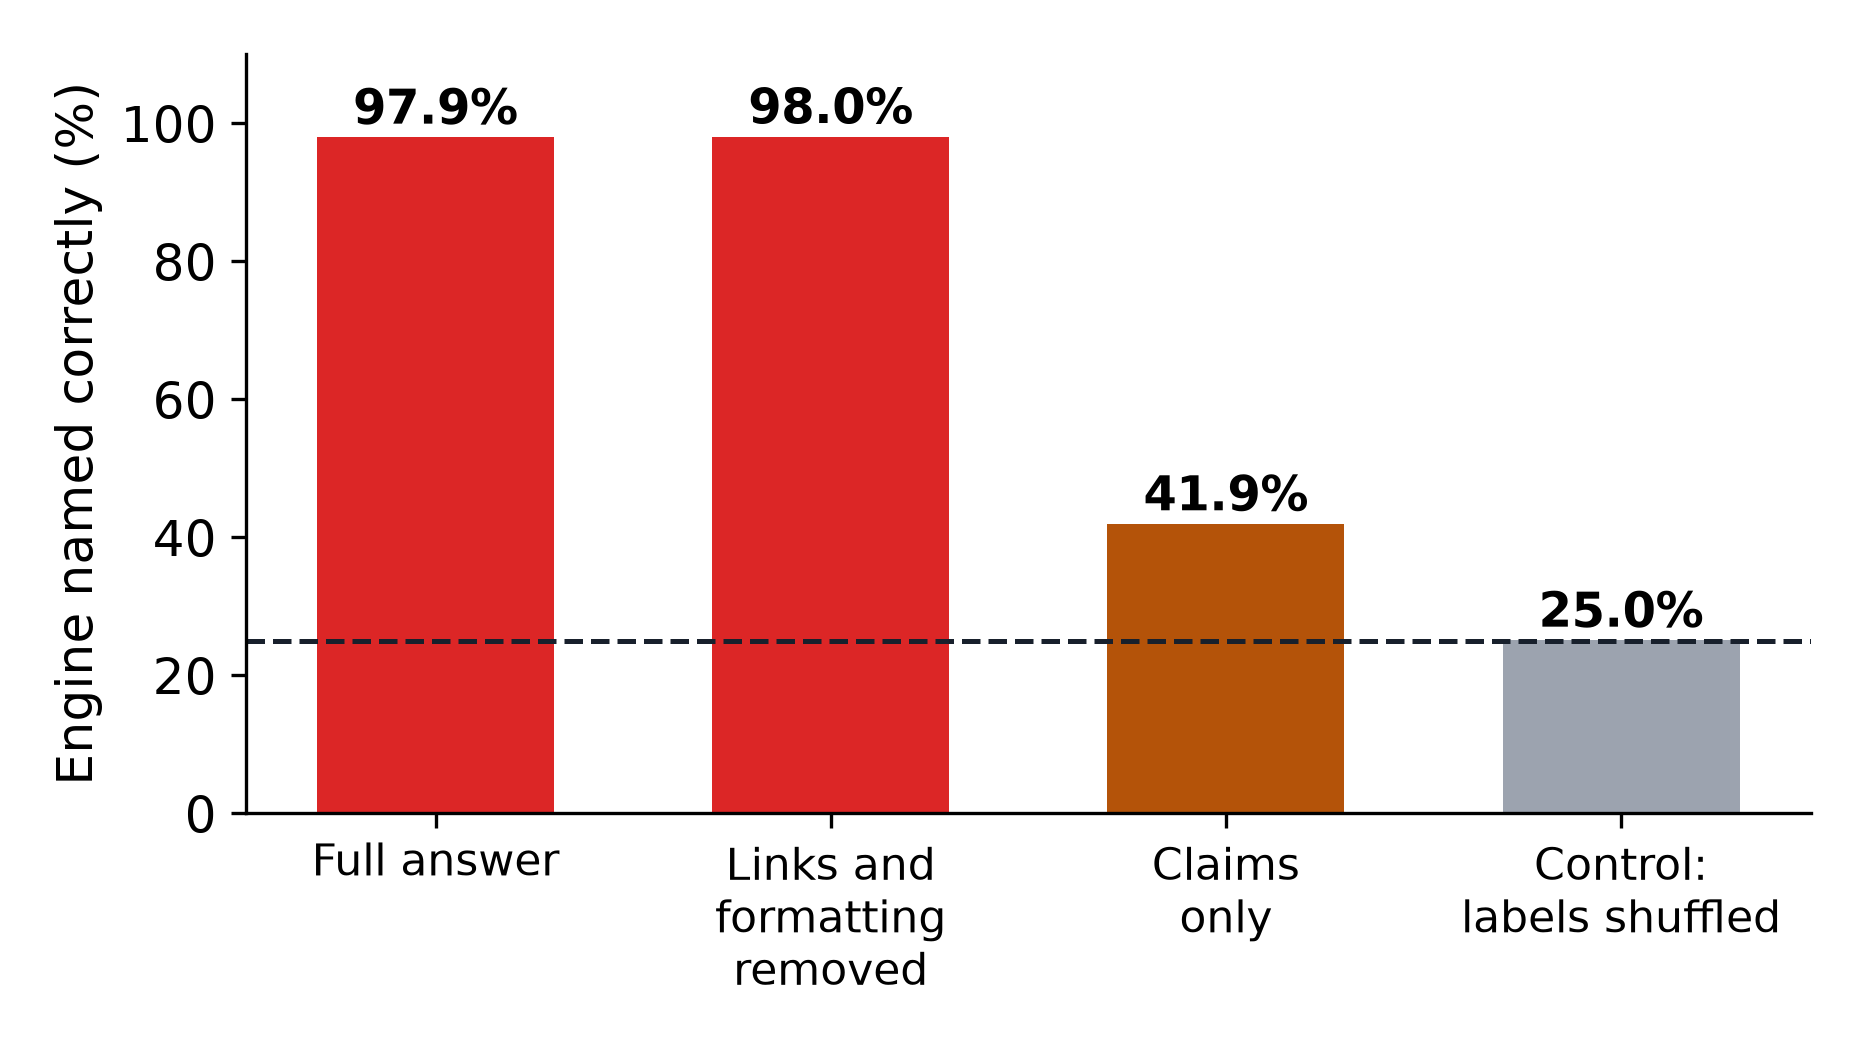
\includegraphics[width=0.8\linewidth]{identity_leak.png}
\caption{Engine identification accuracy by input view. The dashed line is chance (25\%).}
\label{fig:leak}
\end{figure}

\subsection{Self-preference}
\label{sec:pref}

Table~\ref{tab:pref} and Figure~\ref{fig:pref} give each matchup. The Gemini judge picked Gemini's answer in 87.5\% and 90.8\% of comparisons against its two rivals, where the third-family judge picked the same answer in 39.6\% and 37.9\%. The ChatGPT judge picked ChatGPT's answer in 89.2\% and 90.0\% of comparisons, against 60.4\% and 67.1\% under the third-family judge. Averaged over opponents, self-preference was $+50$ points [45, 56] for Gemini, $+26$ [20, 32] for ChatGPT and $-6$ [$-12$, 0] for Claude. Against Gemini, the Claude judge rated Claude's answer 17 points lower than the ChatGPT judge did. Claude chose the first-shown answer in 59.9\% of comparisons and the other two judges in 53.5\%; presenting both orders cancels this position bias.

\begin{table}[t]
\centering
\caption{Win rate of a family's answer under its own judge and under the third family's judge (120 questions, both orders), and their difference with a 95\% bootstrap interval.}
\label{tab:pref}
\begin{tabular}{lccc}
\toprule
Matchup & Own-family judge & Third-family judge & Self-preference \\
\midrule
Gemini answer vs Claude & 90.8\% & 37.9\% (ChatGPT) & $+53$ [45, 62] \\
Gemini answer vs ChatGPT & 87.5\% & 39.6\% (Claude) & $+48$ [40, 56] \\
ChatGPT answer vs Claude & 90.0\% & 67.1\% (Gemini) & $+23$ [16, 30] \\
ChatGPT answer vs Gemini & 89.2\% & 60.4\% (Claude) & $+29$ [20, 37] \\
Claude answer vs ChatGPT & 37.9\% & 32.9\% (Gemini) & $+5$ [$-3$, 13] \\
Claude answer vs Gemini & 45.4\% & 62.1\% (ChatGPT) & $-17$ [$-25$, $-8$] \\
\bottomrule
\end{tabular}
\end{table}

\begin{figure}[t]
\centering
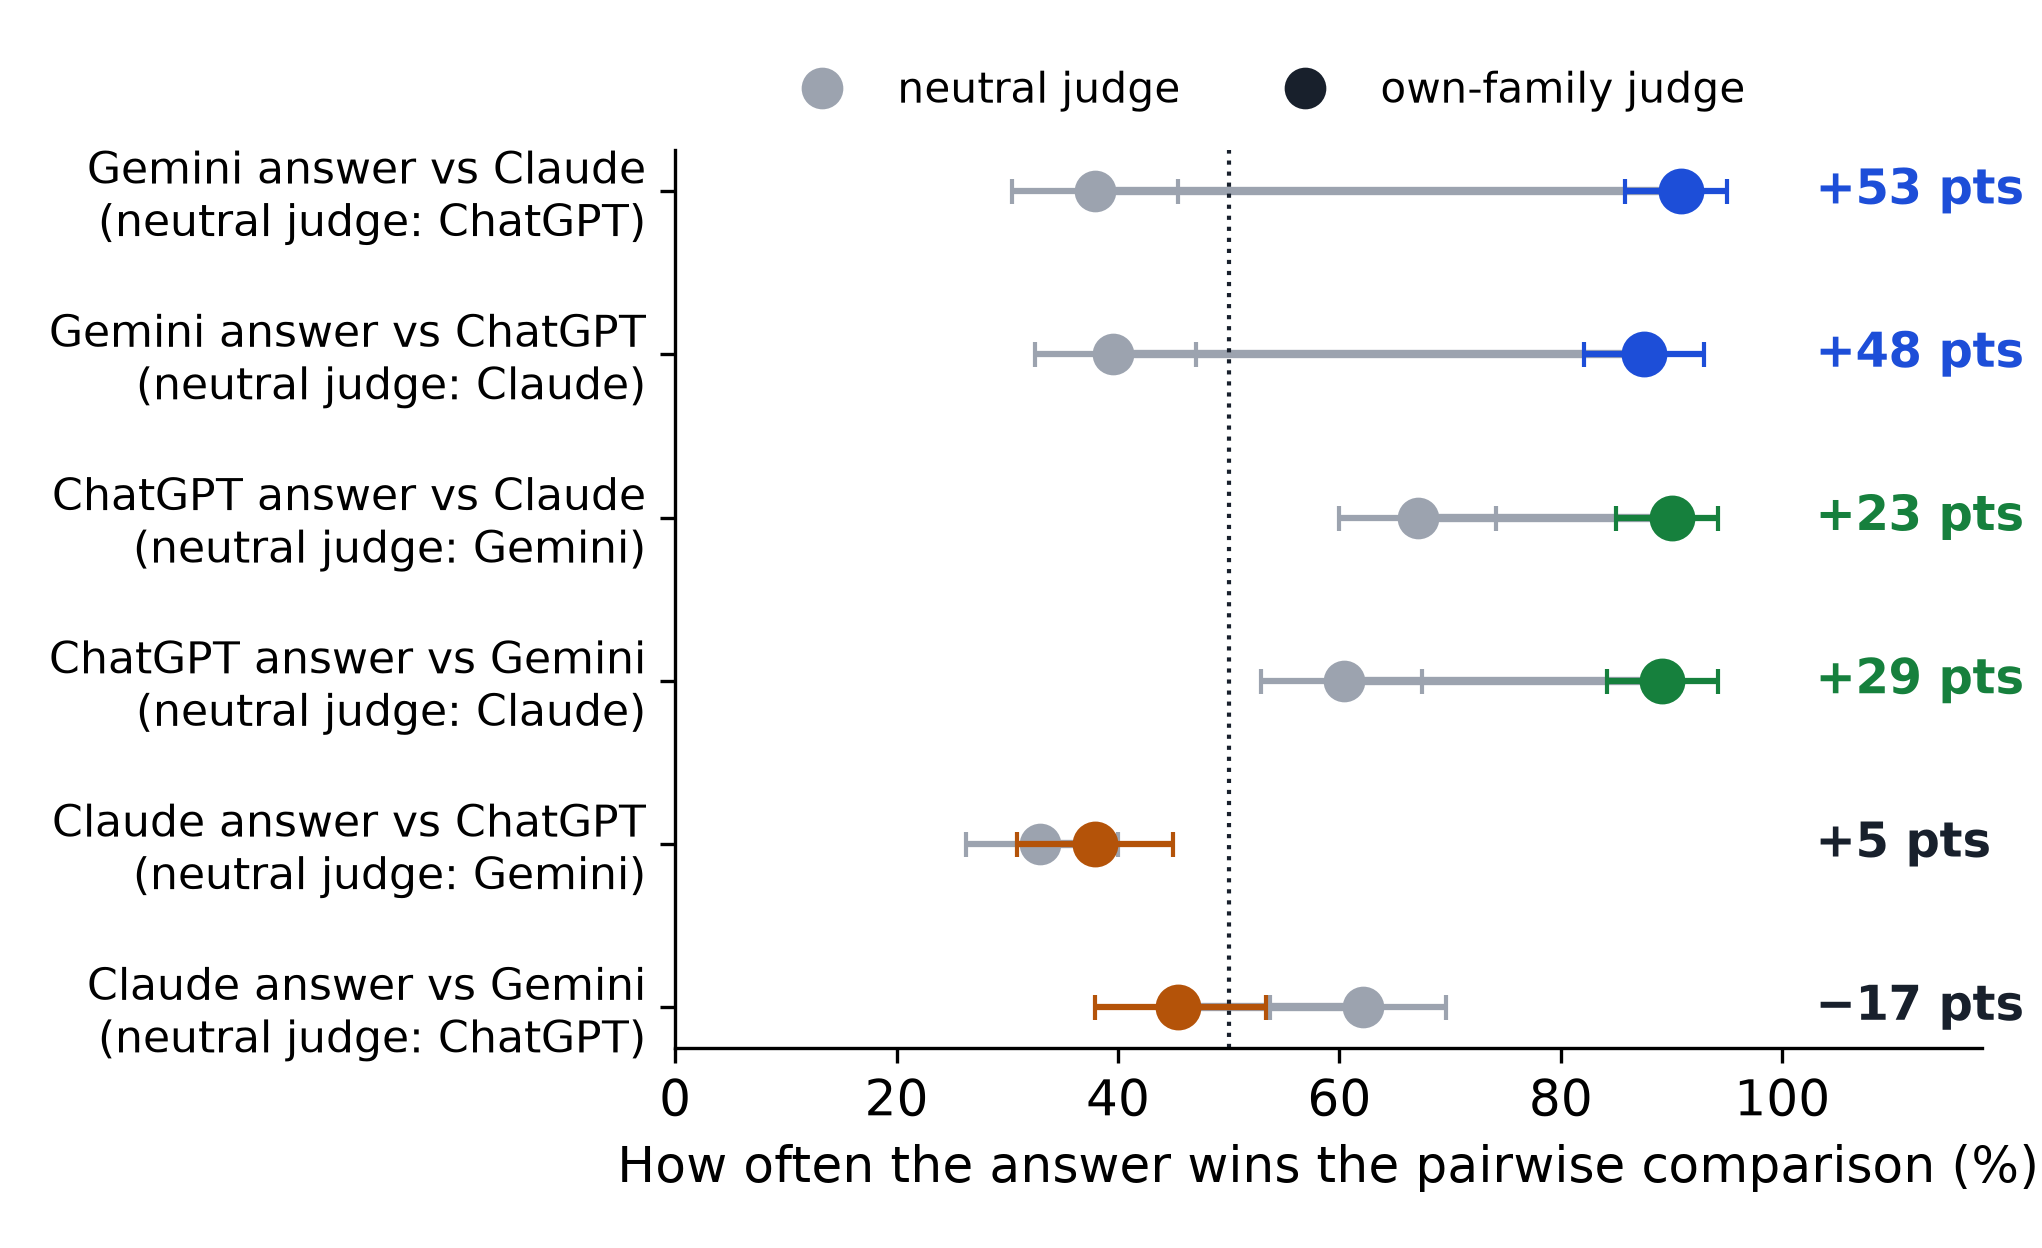
\includegraphics[width=\linewidth]{self_preference.png}
\caption{Win rate of each family's answer under its own judge (colored) and the third family's judge (grey), with 95\% intervals; labels give the difference.}
\label{fig:pref}
\end{figure}

With the second judge of each family, on the 45 to 47 questions completed, self-preference was $+37$ [28, 46] for \texttt{gemini-3.1-pro-preview}, $+29$ [18, 39] for \texttt{gpt-5.6-sol} and $-12$ [$-21$, $-3$] for \texttt{claude-opus-5}.

\subsection{Self-recognition}
\label{sec:recog}

Told that one of two answers is its own, the Gemini judge picked its own in 92.5\% of judgments [89.4, 95.2], the ChatGPT judge in 84.6\% [80.6, 88.3] and the Claude judge in 43.3\% [40.0, 46.5] (Figure~\ref{fig:recog}).

\begin{figure}[t]
\centering
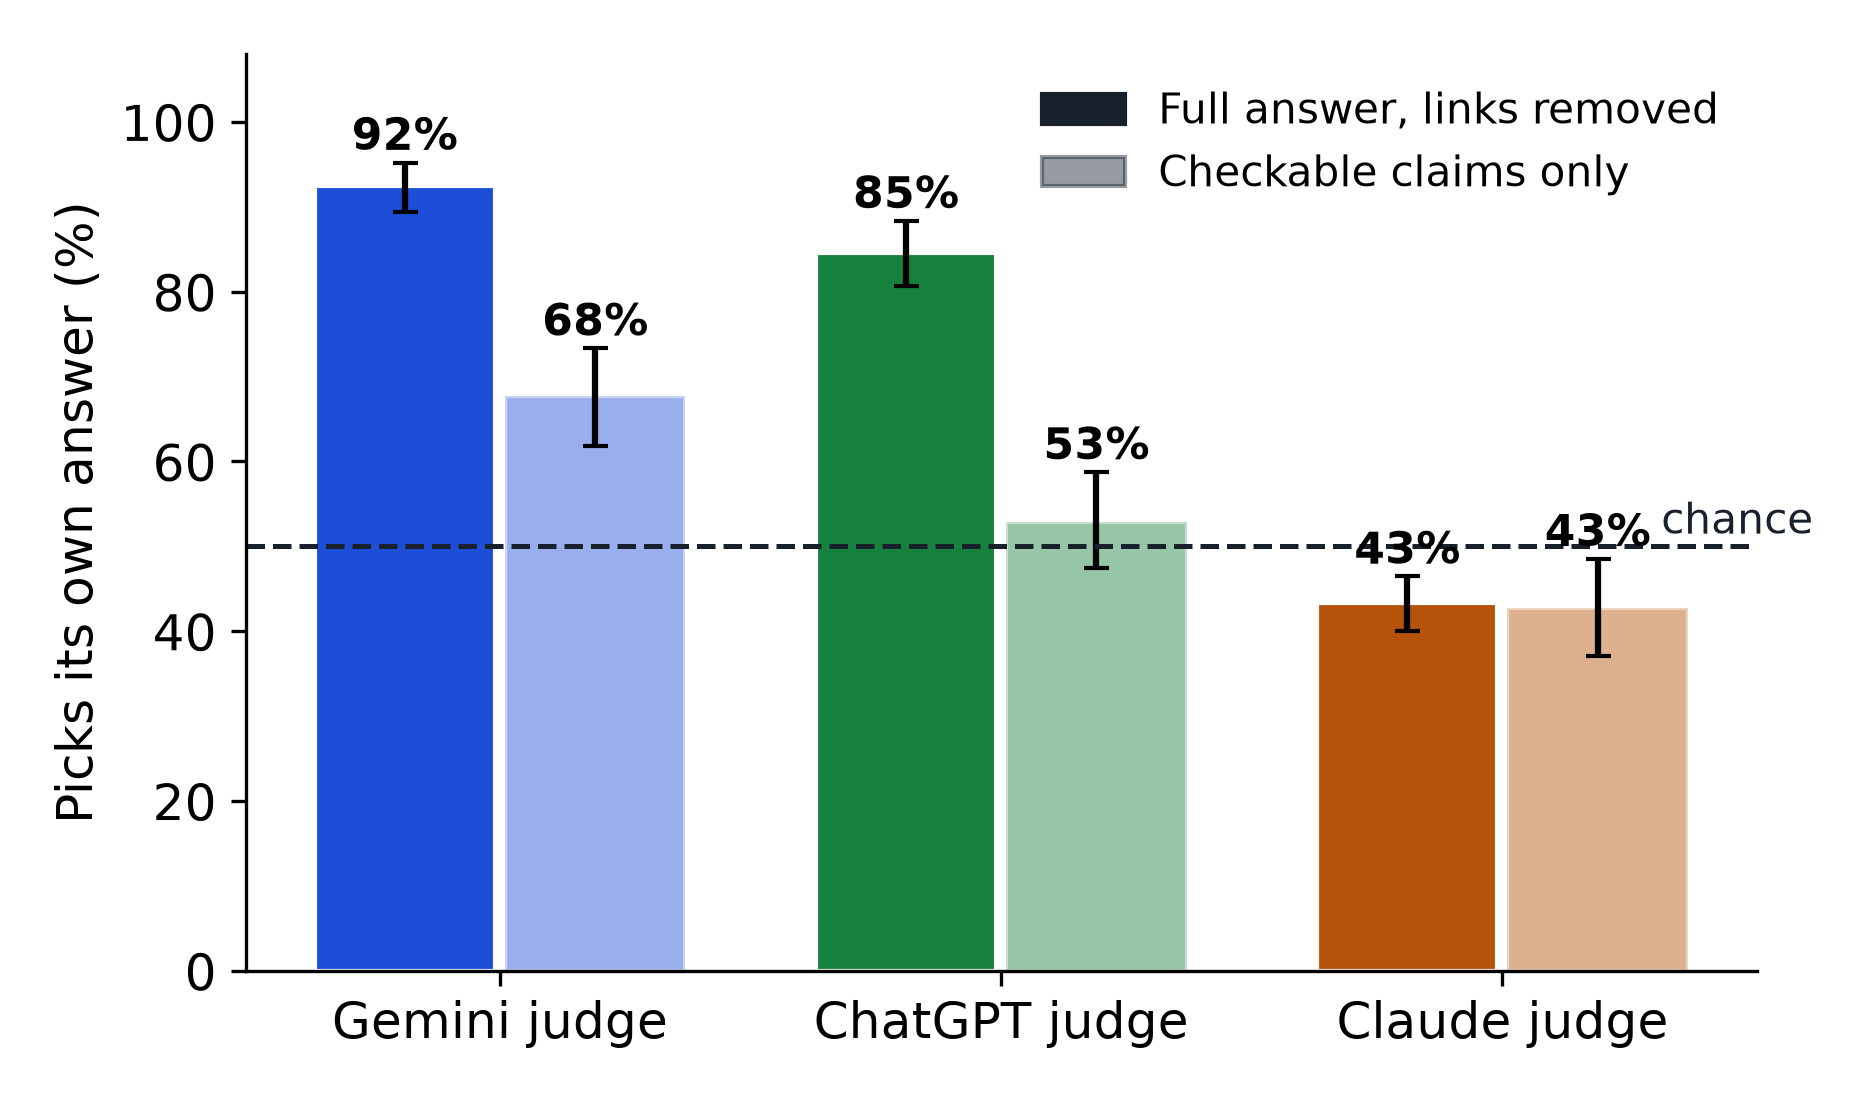
\includegraphics[width=0.8\linewidth]{self_recognition.png}
\caption{Share of judgments in which a judge, told that one of two answers is its own, picks its own, from the full answer and from the claims only. The dashed line is chance (50\%).}
\label{fig:recog}
\end{figure}

\subsection{Input views}
\label{sec:views}

The rewriter kept on average 99.0\% of each answer's checkable claims, and all of them in 95.6\% of the 360 answers. Table~\ref{tab:views} and Figure~\ref{fig:mitig} compare the three views. On rewritten answers, recognition was 83.1\% for Gemini and 85.6\% for ChatGPT, and self-preference was $+49$ [43, 54] and $+27$ [22, 33]. On claims only, recognition was 67.7\% and 52.9\%, and self-preference was $+24$ [17, 31] and $+7$ [1, 12]. Claude's recognition stayed between 42.7\% and 44.8\% and its self-preference between $-8$ and $-6$ in all views. Across the nine combinations of judge and view, the Pearson correlation between recognition and self-preference was 0.94 (Figure~\ref{fig:rvp}).

\begin{table}[t]
\centering
\caption{Self-recognition (judge picks its own answer; chance 50\%) and self-preference (points, 95\% bootstrap interval) by input view.}
\label{tab:views}
\begin{tabular}{llccc}
\toprule
Judge & Measure & Full answer & Rewritten & Claims only \\
\midrule
Gemini & recognition & 92.5\% & 83.1\% & 67.7\% \\
       & preference & $+50$ [45, 56] & $+49$ [43, 54] & $+24$ [17, 31] \\
ChatGPT & recognition & 84.6\% & 85.6\% & 52.9\% \\
        & preference & $+26$ [20, 32] & $+27$ [22, 33] & $+7$ [1, 12] \\
Claude & recognition & 43.3\% & 44.8\% & 42.7\% \\
       & preference & $-6$ [$-12$, 0] & $-6$ [$-12$, $-1$] & $-8$ [$-13$, $-2$] \\
\bottomrule
\end{tabular}
\end{table}

\begin{figure}[t]
\centering
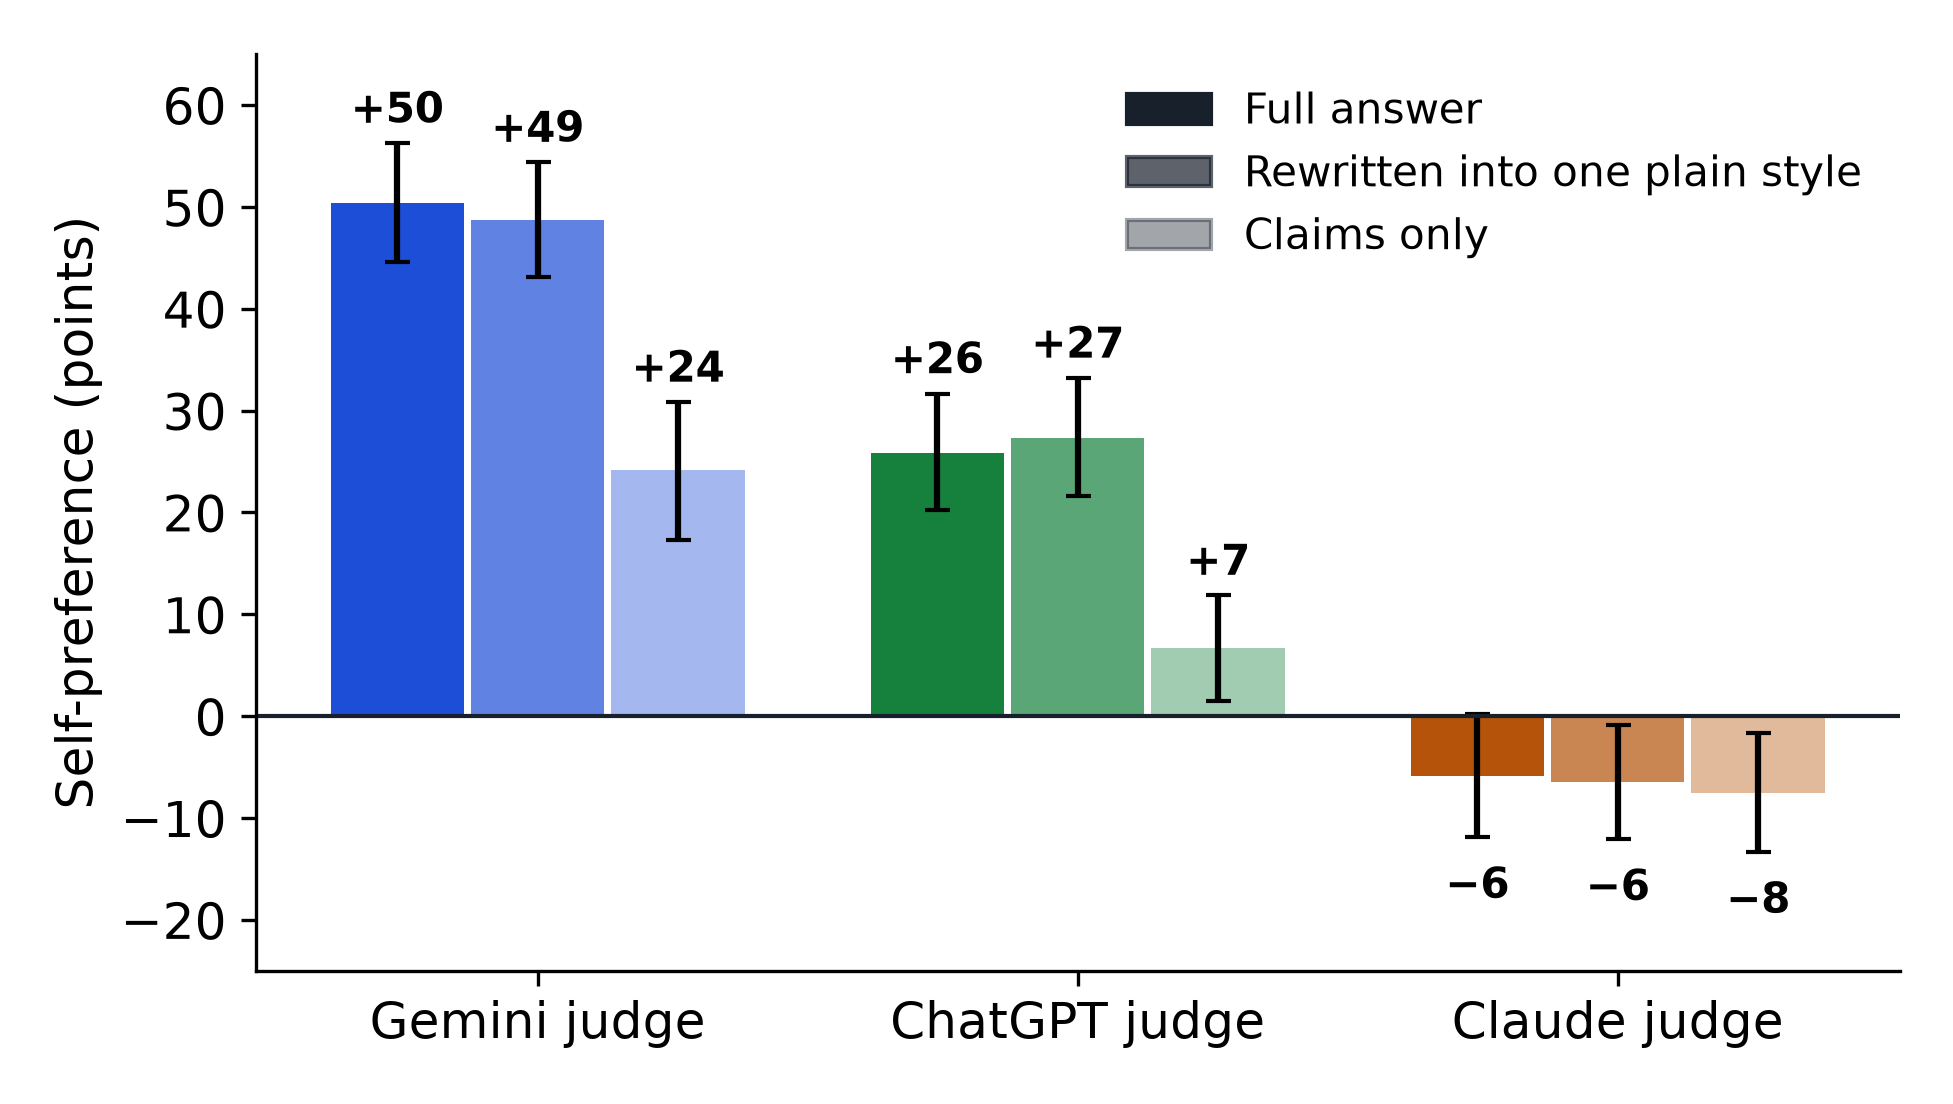
\includegraphics[width=0.85\linewidth]{mitigations.png}
\caption{Self-preference by judge and input view, with 95\% intervals.}
\label{fig:mitig}
\end{figure}

\begin{figure}[t]
\centering
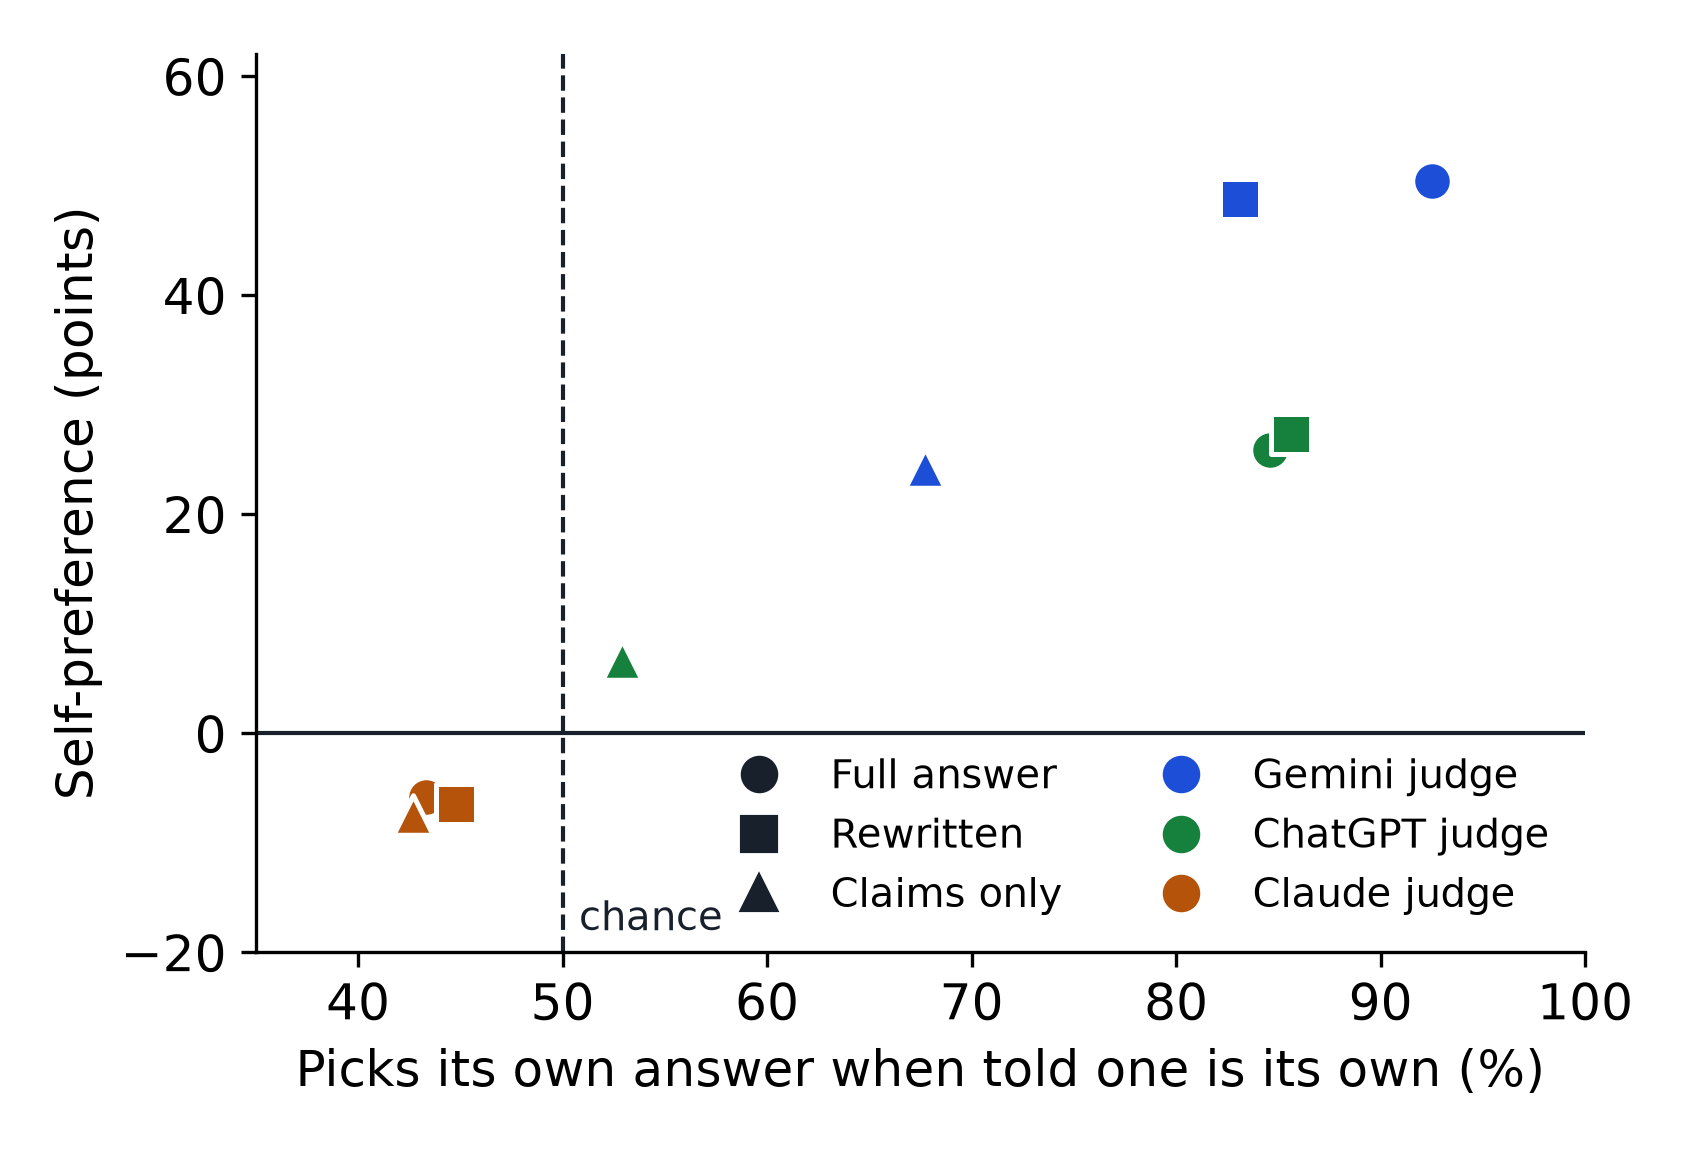
\includegraphics[width=0.7\linewidth]{recognition_vs_preference.png}
\caption{Self-recognition against self-preference for each judge (color) and input view (marker).}
\label{fig:rvp}
\end{figure}

\subsection{Rankings}
\label{sec:rank}

Table~\ref{tab:rank} gives each engine's overall win rate under each judge. The Gemini judge ranked Gemini first and the ChatGPT judge ranked ChatGPT first, each with about 89\% of wins. The Claude judge ranked ChatGPT first and Claude last. Under third-family judges alone, ChatGPT won both of its matchups (67.1\% against Claude, 60.4\% against Gemini) and Claude won against Gemini (62.1\%).

\begin{table}[t]
\centering
\caption{Win rate of each engine's answers under each judge (480 judgments per cell: two matchups, 120 questions, both orders). Bold marks the engine each judge ranks first.}
\label{tab:rank}
\begin{tabular}{lccc}
\toprule
Judge & Claude answers & Gemini answers & ChatGPT answers \\
\midrule
Claude judge & 41.7\% & 47.1\% & \textbf{61.2\%} \\
Gemini judge & 21.0\% & \textbf{89.2\%} & 39.8\% \\
ChatGPT judge & 36.0\% & 24.4\% & \textbf{89.6\%} \\
\bottomrule
\end{tabular}
\end{table}

\section{Discussion}
\label{sec:discussion}

The principal finding is that hiding names did not keep two of three same-family judges from favoring their own family on real answers, and that these two judges could find their own answers. The classifier result in Section~\ref{sec:leak} sets the context: the writer's identity is present in the text, so a pipeline that relies on hidden names has no evidence that its judge cannot see it.

The input views separate two explanations for recognition. If judges recognized themselves by style, a common style should have removed recognition. It did not, and it left self-preference unchanged, whereas removing wording and order while keeping the claims reduced both. We infer that the judges mainly recognize content: which products an answer recommends and which figures it gives. This fits the familiarity account of \citet{wataoka2024self}, under which a judge finds most plausible the content it would itself produce. The co-movement of recognition and preference across views is consistent with the linear relation reported by \citet{panickssery2024llm}; with nine dependent points we treat it as consistency, not as a new estimate.

An alternative explanation deserves weight. A judge may favor its own family's answers because it shares that family's knowledge about products, so that what looks like self-preference is a judge applying its own beliefs about which claims are true. Our design cannot separate this from bias, because it has no ground truth. For a pipeline the consequence is the same either way: a same-family judge does not give an independent check.

The Claude judges are the unexpected result. Neither Claude model recognized or favored Claude's answers, and Claude Sonnet rated them slightly below the third-family judge. We do not have an explanation, and the result may not hold for other prompts, tasks or versions. For the source study, it means its choice of a Claude judge did not inflate Claude's results on our measurements. The cross-vendor spot-check that the study also ran is the step where the effect we measured matters, because a Gemini or ChatGPT judge favors its own family on these answers.

Two checks follow, and both can be run in code. The first is that no family judges a comparison that contains its own answer. With three or more families a judge from a family that wrote neither answer is always available, which applies the multi-family panel of \citet{verga2024replacing} at the level of each comparison; the rankings in Section~\ref{sec:rank} show what happens without it. The second is to give judges extracted claims rather than prose when the judgment concerns factual reliability. Because the claims view reduced but did not remove the largest preference, it complements the first check and does not replace it. A self-recognition test, at four judgments per item, can show before deployment which judges need the first check.

\section{Limitations}
\label{sec:limits}

The judgments are preferences without ground truth, so self-preference is measured against a third-family judge that has its own preferences. A ground-truth test, in which one of two answers is known to be correct, would show whether the preference also selects wrong answers; we planned it and did not run it. We used one prompt of our own rather than the source study's rubric, which classifies conflicts among 40 answers at once, and self-preference may differ under that rubric; rerunning the measurement with the rubric would settle this. The judge experiments used free-tier answers, one sample per configuration and 120 of the 217 scored questions, and Perplexity, which has no matching judge model, appears only in the classifier. The second-judge estimates rest on 45 to 47 questions per family and their intervals are 1.5 to 1.8 times as wide as in the main run. The source study does not name the Claude version it used as a judge, so our Claude results describe the two Claude models we tested.

\section{Conclusion}
\label{sec:conclusion}

Hiding which system wrote an answer did not stop two of three LLM judges from favoring their own family on a published set of real shopping answers, and the same two judges could pick out their own answers. Putting every answer into one style left the preference in place; stripping answers down to their claims cut it by half or more. A pipeline that compares systems should therefore keep each judge away from comparisons involving its own family, and should test its judges for self-recognition before relying on them. The next step is the two measurements named in Section~\ref{sec:limits}: a ground-truth test that shows whether the preference also selects wrong answers, and a rerun under the source study's own rubric.

\section*{Declaration of generative AI use}
The author used Claude (Anthropic), an AI assistant, during this work: to write and debug the data-processing and API-calling code, to draft and edit the text, and to search for and check references. The author defined the aims of the study, approved the experimental design, checked every reported number against the released result files and every reference against its source, and takes full responsibility for the content. Because Claude is also one of the model families studied, we note that the assistant did not act as a judge in any experiment: every judgment comes from an API call recorded in the released per-call files.

\section*{Competing interests}
The author has no employment, funding or other financial relationship with Product.ai, Anthropic, Google, OpenAI or Alibaba. The API costs were paid by the author.

\section*{Funding}
This work received no funding.

\section*{Data and code availability}
The answers are the source study's dataset, released under CC BY 4.0 \citep{productai2026divergence}. The code (MIT license), the per-call records of all 12,007 judge and rewriter calls (judge, returned model, choice and cost), the result files and the figures are at \url{https://github.com/vahit19/verdict-gate/tree/main/studies/judge_self_preference}. The main run cost 9.51 USD and the follow-up runs 18.75 USD.

\bibliography{refs}
\bibliographystyle{tmlr}

\appendix
\section{Prompts}
\label{app:prompts}

\paragraph{Pairwise preference.} \emph{A shopper asked an AI shopping assistant the question below on 2026-09-01. Two assistants answered. Judge which answer is more factually reliable for the shopper: correct and current products, specs and prices, and no unsupported claims. Ignore length, tone and formatting.} The question and the two answers follow, then \emph{Reply with only JSON: \{"winner": "A"\} or \{"winner": "B"\}.} In the rewritten view the second sentence is followed by \emph{Both answers were rewritten into the same plain style by a third system; their content is unchanged.} In the claims view it is followed by \emph{Each answer is shown only as the list of checkable items it mentioned (prices, model numbers, numbers with units).}

\paragraph{Self-recognition.} \emph{Below are two answers to the same shopping question. Exactly one of them was written by you, the model reading this, in a separate session. The other was written by a different AI system.} The rewritten and claims views add the sentence given above for that view. The question and the two answers follow, then \emph{Which answer did you write? Reply with only JSON: \{"mine": "A"\} or \{"mine": "B"\}.}

\paragraph{Rewriting.} \emph{Rewrite the shopping answer below in plain, neutral prose. Keep every product name, model number, price, number, recommendation and claim exactly as stated, including any that may be wrong. Do not add, remove, correct or soften anything. Use plain paragraphs: no markdown, no headings, no bullet points, no bold, no links, no emoji. Do not mention that this is a rewrite. Keep a similar length.}

\end{document}
